\begin{figure}[htbp]
\centering
\captionsetup{
  justification=raggedright,
  labelsep=none,
  singlelinecheck=false,
  labelformat=boldlabel,
}
\caption[Figure 8: \footnotesize ]{\footnotesize \textbf{: Selected hyperparameters over time.} Bayesian-tuned hyperparameter values chosen at each walk-forward refit, for every tuned ML model (GLMNET, RF, XGB, NN1--NN3; OLS is untuned and omitted). Hyperparameters that play the same role across models share a panel and are drawn as separate coloured lines: number of trees (RF num.trees, XGB nrounds), maximum tree depth, minimum leaf size (RF min.bucket, XGB min\_child\_weight), learning rate (XGB eta, NN lr), early-stopping iteration and feature subsampling (RF mtry, XGB colsample\_bytree; both fractions of the features sampled). Model-specific hyperparameters keep their own panels, and the three neural networks share each remaining NN panel. Points are the selected values at each refit date; vertical scales differ across panels. Estimated on the individual-signals run.}
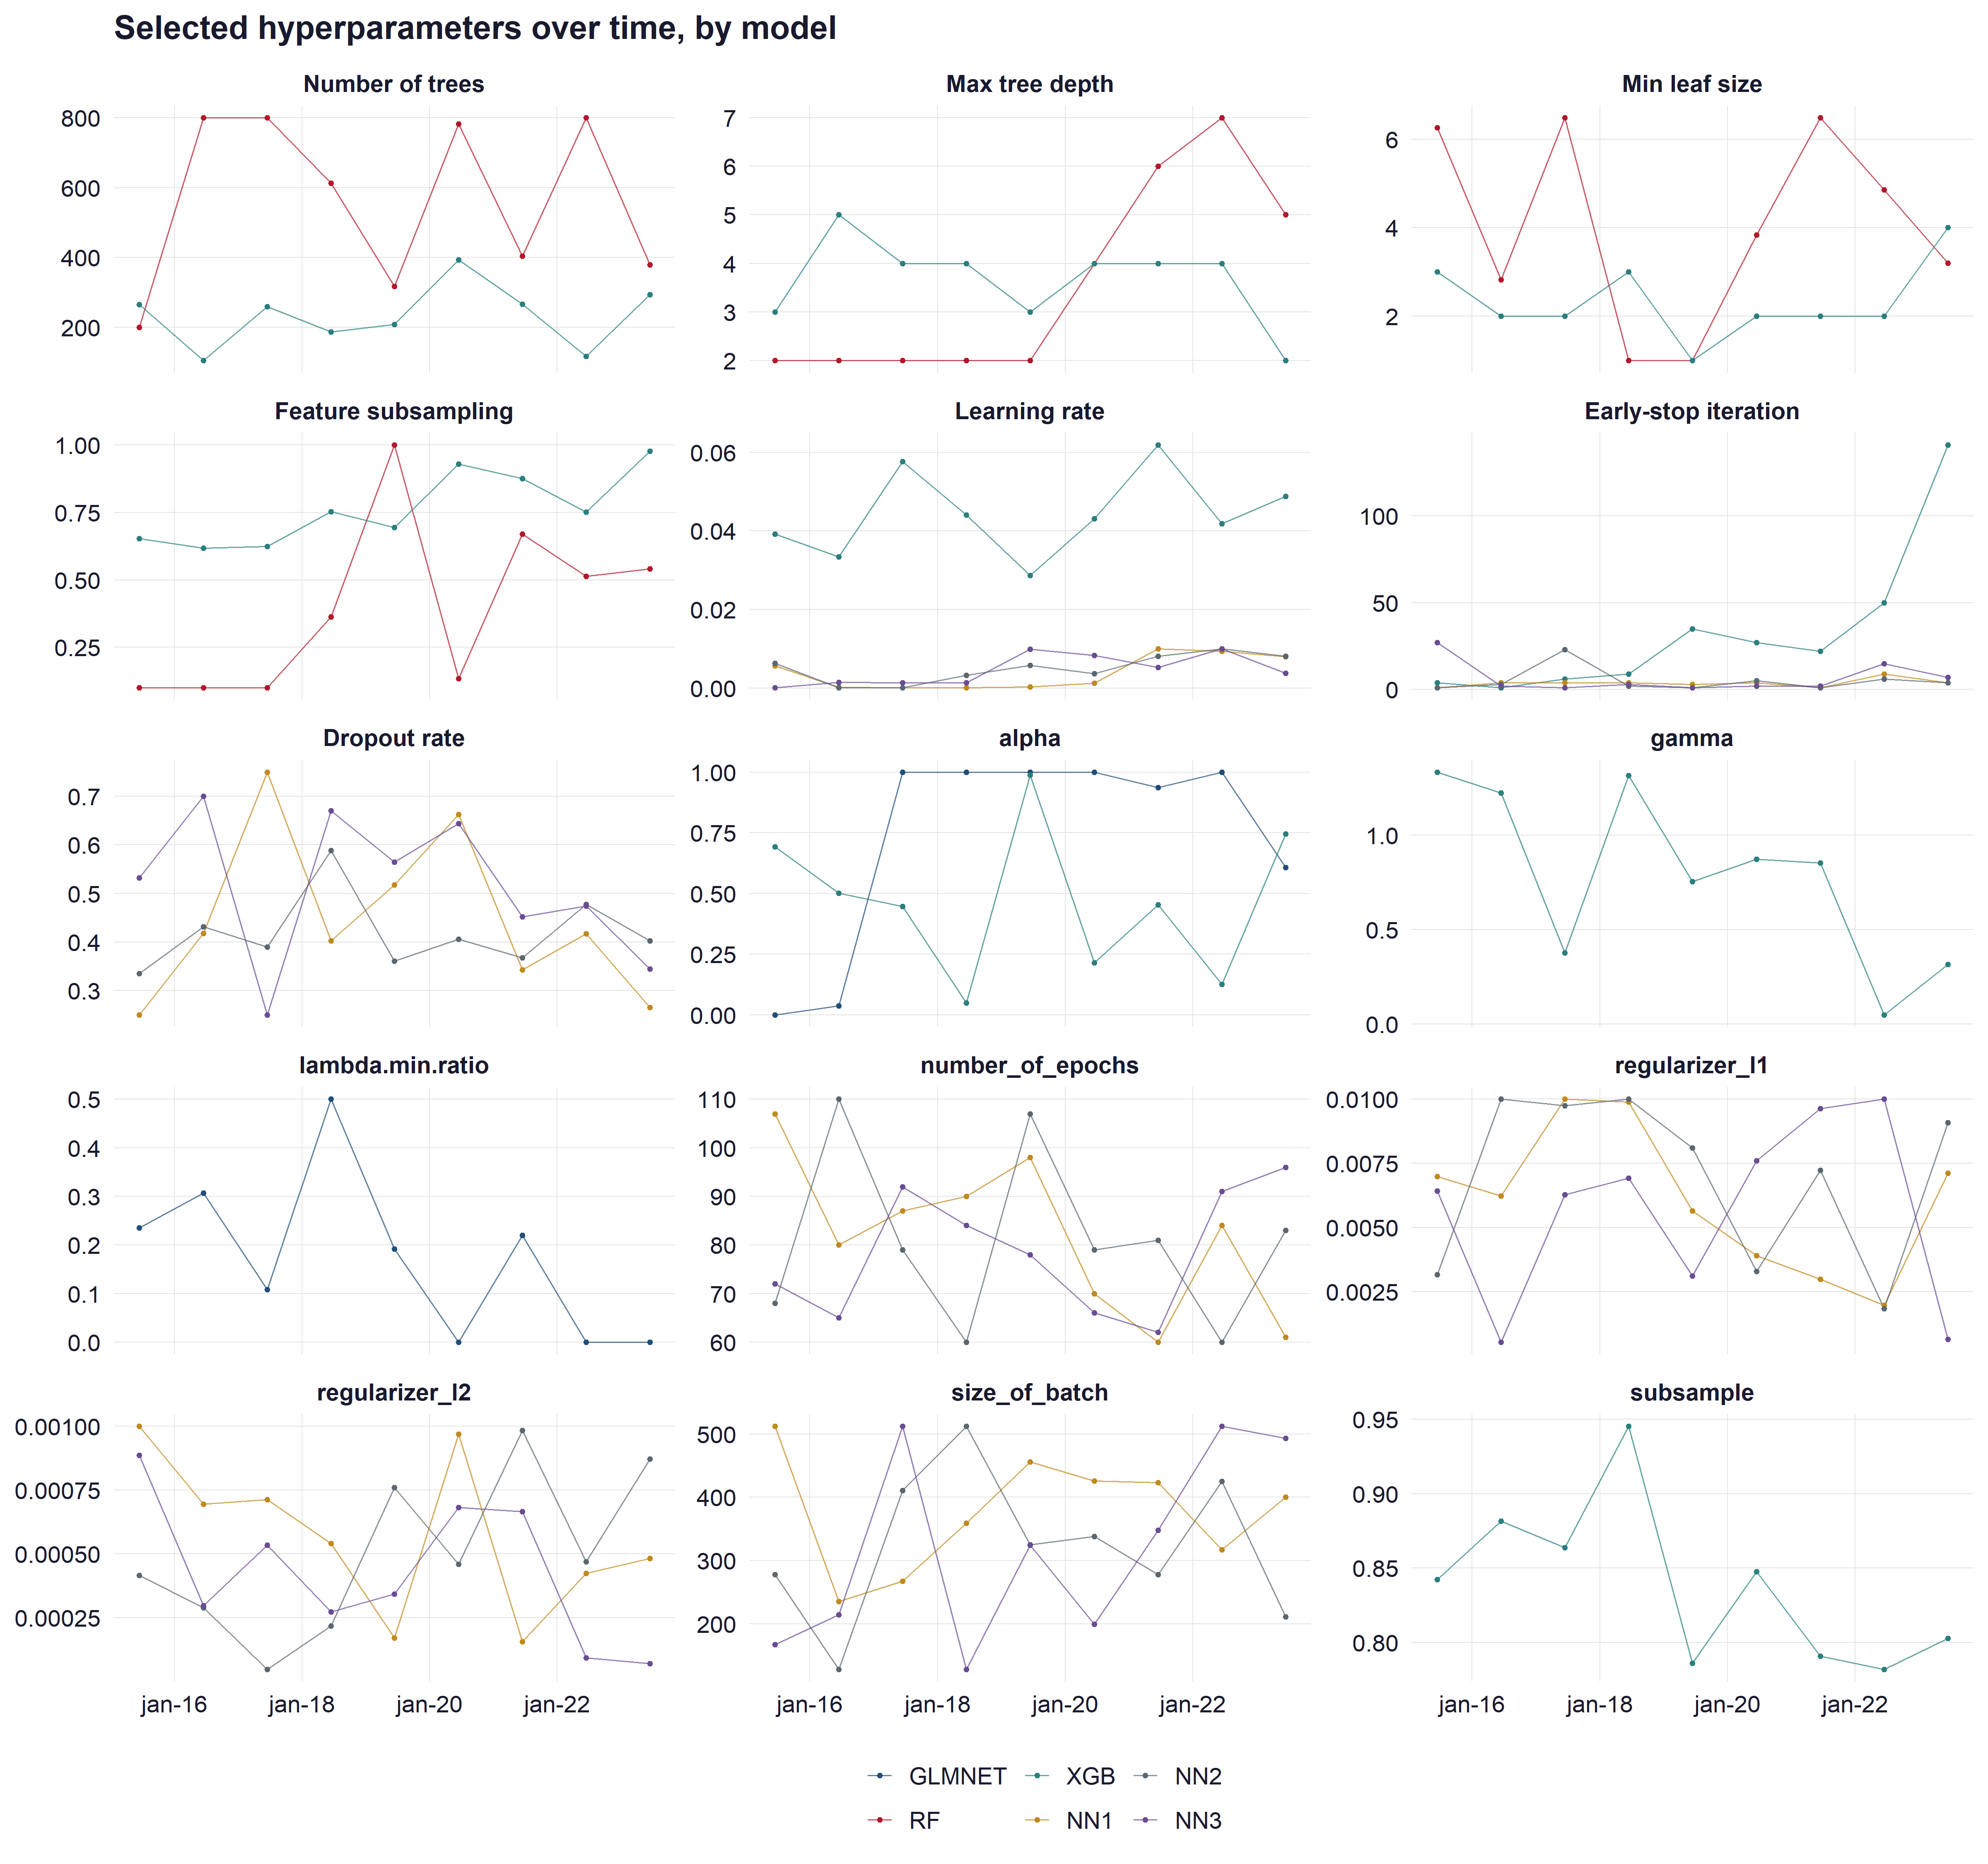
\includegraphics[width=\linewidth]{figures/hyperparameters_over_time.png}
\label{fig:hyper_time}
\end{figure}
